\chapter{Enterprise Architecture}

\section{Definition}

Die Unternehmensarchitektur als Disziplin umfasst Prinzipien und Methoden, um Geschäfts- und IT Architektur eines Unternehmens zu entwerfen und umzusetzen. Sie stellt den Zusammenhang zwischen der Geschäfts- und der IT Architektur her.

\begin{figure}[h!]
\centering
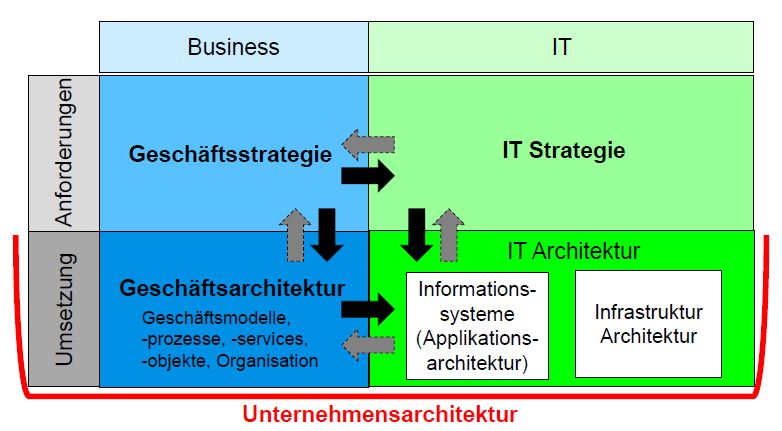
\includegraphics[width=0.7\linewidth]{fig/unternehmensarchitektur}
\caption{Zusammenhang Strategie und Architektur}
\label{fig:unternehmensarchitektur}
\end{figure}

Die Geschäftsarchitektur befasst sich mit den Zielen, Fassaden, interner und externer Kommunikation sowie Prozesse und Geschäftsentitäten.

\begin{figure}[h!]
\centering
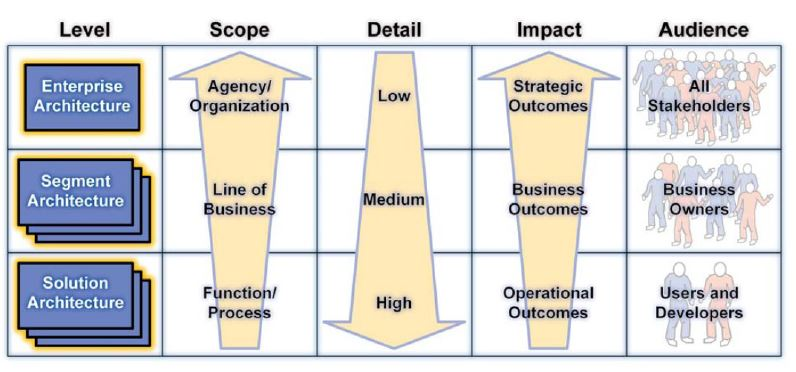
\includegraphics[width=0.7\linewidth]{fig/ea-vs-application}
\caption{EA im Vergleich zur Applikationsarchitektur}
\label{fig:ea-vs-application}
\end{figure}

Die Hauptaufgaben der Unternehmensarchitektur sind: Anwendungslandschaften gestalten, Bebauungsplan sowie Standardisierung. Mögliche Ziele für die Gestaltung der Anwendungslandschaft sind:

\begin{itemize}
	\item Konsolidierung/Reduktion von Heterogenität durch Standardisierung
	\item Fusionsmanagement (Konsolidierung)
	\item Verbesserung von Ertragskraft und Kostenmanagement
		\subitem Prozessautomatisierung, Kundenselbstbedienung
		\subitem Zerlegung von Geschäftsprozessen
		\subitem Umsetzung unternehmensübergreifender IT-Prozesse
		\subitem IT Kosten Reduktion
	\item Verbesserung Time-To-Market
	\item Verbesserung Kundenzufriedenheit
	\item Auslagerung von Geschäftsprozessen, Infrastruktur, Anwendungen
\end{itemize}

\section{Sichten}

\subsection{Clusterkarte}

Eine Clusterkarte fasst die Systeme eines Unternehmens (z.B. Services oder Datenbanken) in logische Domänen zusammen. Die Domänen ergeben sich aus Funktionsbereichen, Organisationseinheiten oder Standorten.

\begin{figure}[h!]
\centering
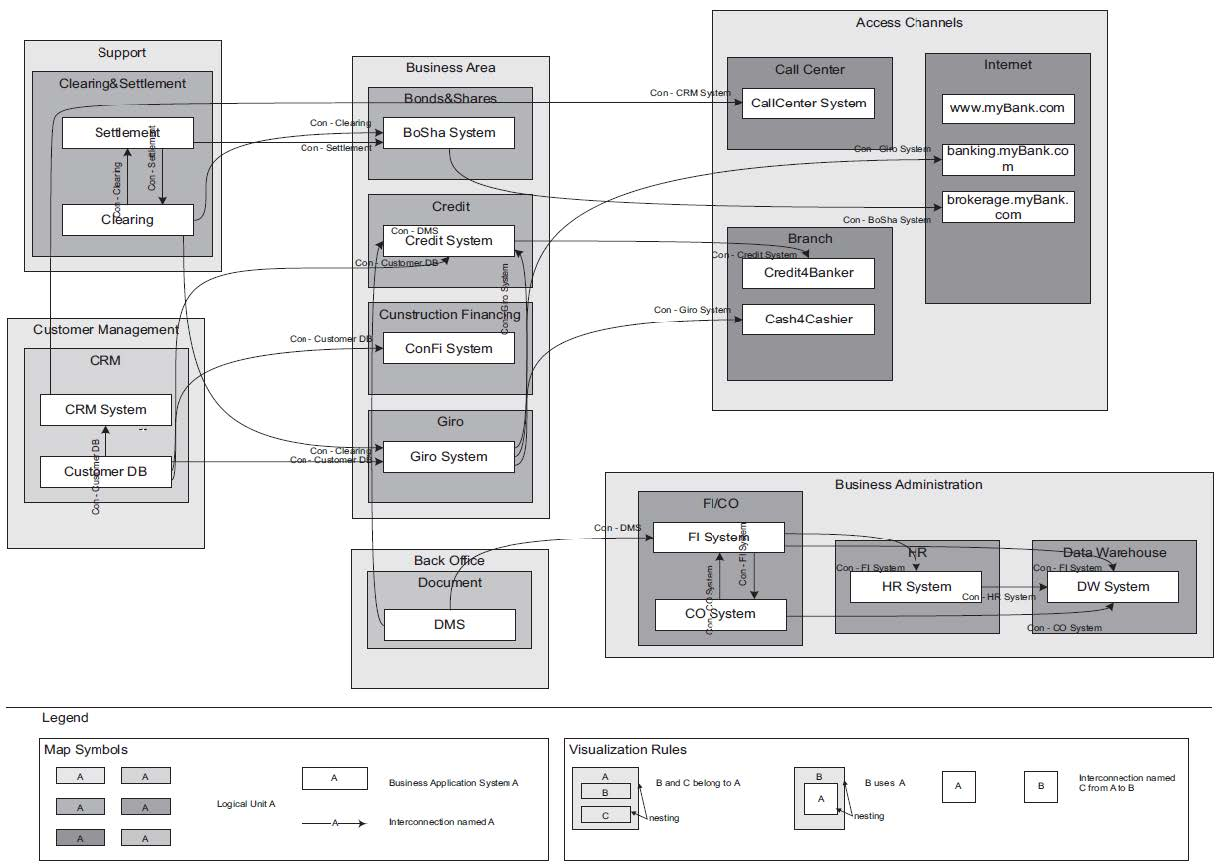
\includegraphics[width=\linewidth]{fig/clusterkarte}
\caption{Clusterkarte}
\label{fig:clusterkarte}
\end{figure}

\subsection{Prozessunterstützungskarte}

Bei der Prozessunterstützungskarte wird auf der X-Achse die Wertschöpfungskette des Unternehmens dargestellt. Auf der Y-Achse sind z.B. die Organisationseinheiten oder Produkte aufgelistet. Innerhalb der Karte werden die physischen oder logischen IT-Systeme angeordnet. Sie dienen dazu gewachsene Anwendungslandschaften zusammenzuführen.

\begin{figure}[h!]
\centering
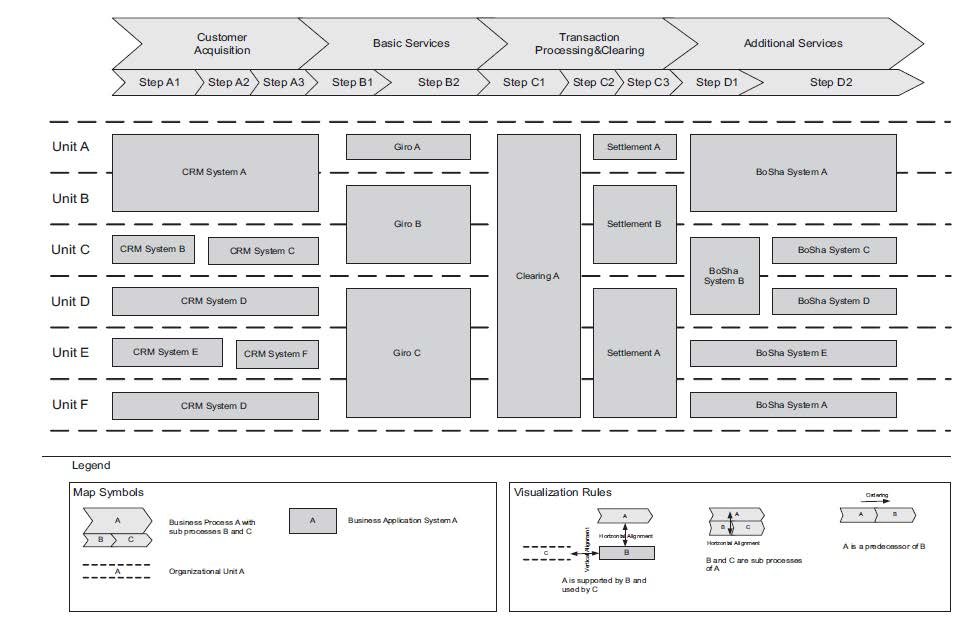
\includegraphics[width=\linewidth]{fig/prozessunterstuetzungskarte}
\caption{Prozessunterstützungskarte}
\label{fig:prozessunterstuetzungskarte}
\end{figure}

\subsection{Intervallkarte}

Eine Intervallkarte zeigt wie sich die Anwendungssysteme über die Zeit entwickeln. Jede Version einer Anwendung wird mit ihrem Status auf einem Zeitstrahl abgebildet.

\begin{figure}[h!]
\centering
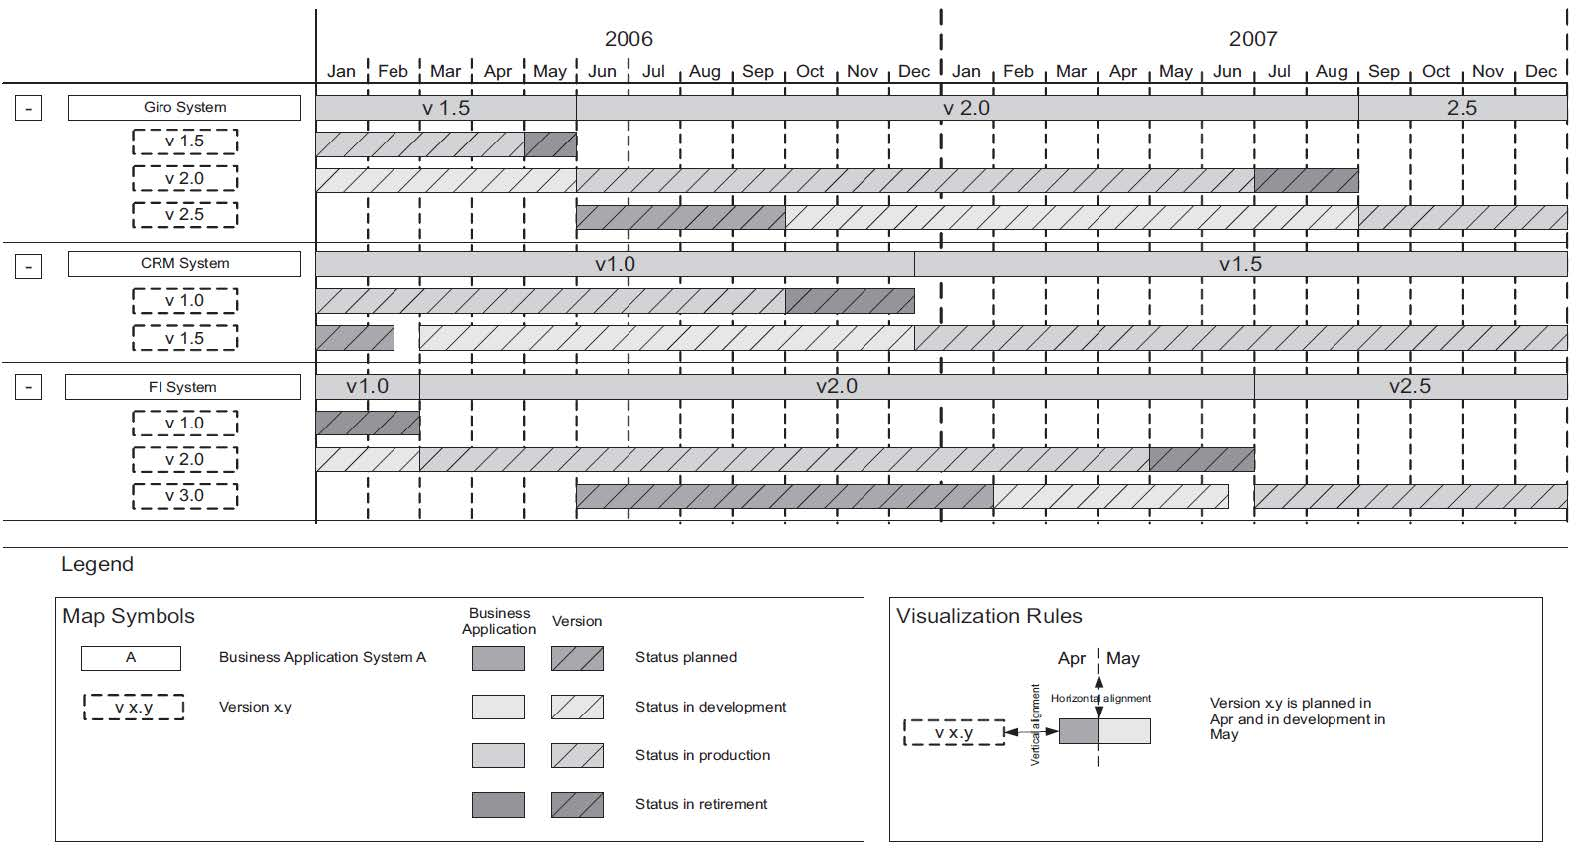
\includegraphics[width=\linewidth]{fig/intervallkarte}
\caption{Intervallkarte}
\label{fig:intervallkarte}
\end{figure}

\section{Enterprise Architecture Frameworks}

Enterprise Architektur Frameworks beschreiben folgendes:
\begin{itemize}
	\item Thematisierung des Zusammenhangs von Business und IT
	
	\item Definition von Begriffen/Modellen zur Beschreibung der Architektur
	
	\item Unterscheidung verschiedener Ebenen und Sichten der Geschäfts- und IT Architektur
	
	\item Beschreibung von Geschäftsprozessen und -services und ihre Abbildung in der IT
\end{itemize}

\subsection{Zachmann}

\textit{With increasing size and complexity of the implementations of information systems, it is necessary to use some logical construct (or architecture) for defining and controlling the interfaces and the integration of all the components of a system.} - John Zachmann bereits 1987.

Architektur ist relativ und es gibt nicht nur eine Lösung. Dieser Umstand erschwert auch die Kommunikation der Architektur. Die Architekturen sind jeweils additiv und komplementär.

Das Framework nach Zachman ist ein Klassiker und hält sich. Er teilt die Architektur nach Architekturebenen (Business, Informationssysteme, Technologie) sowie nach Architektur-Sichten (Daten, Prozesse, Netzwerke) ein.

\begin{figure}[h!]
\centering
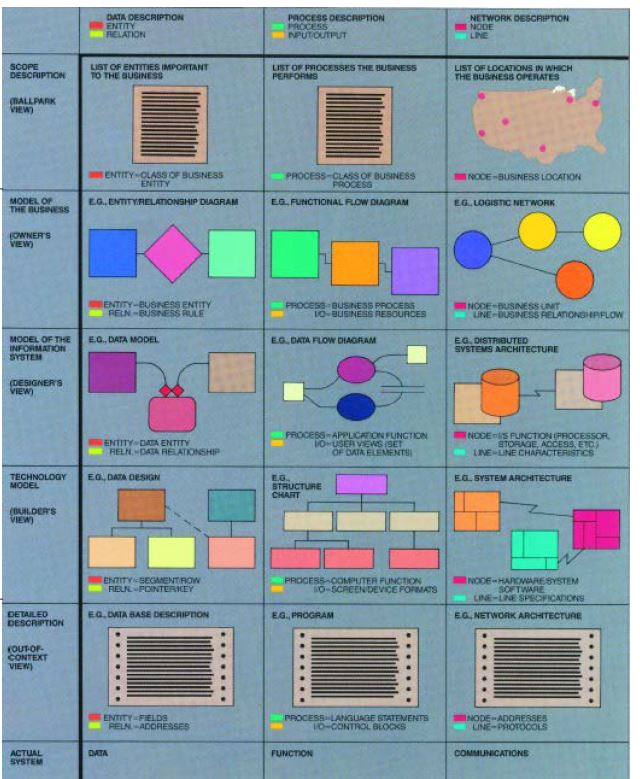
\includegraphics[width=0.7\linewidth]{fig/zachmann-model}
\caption{Architektur Framework Zachmann}
\label{fig:zachmann-model}
\end{figure}

\begin{figure}[h!]
\centering
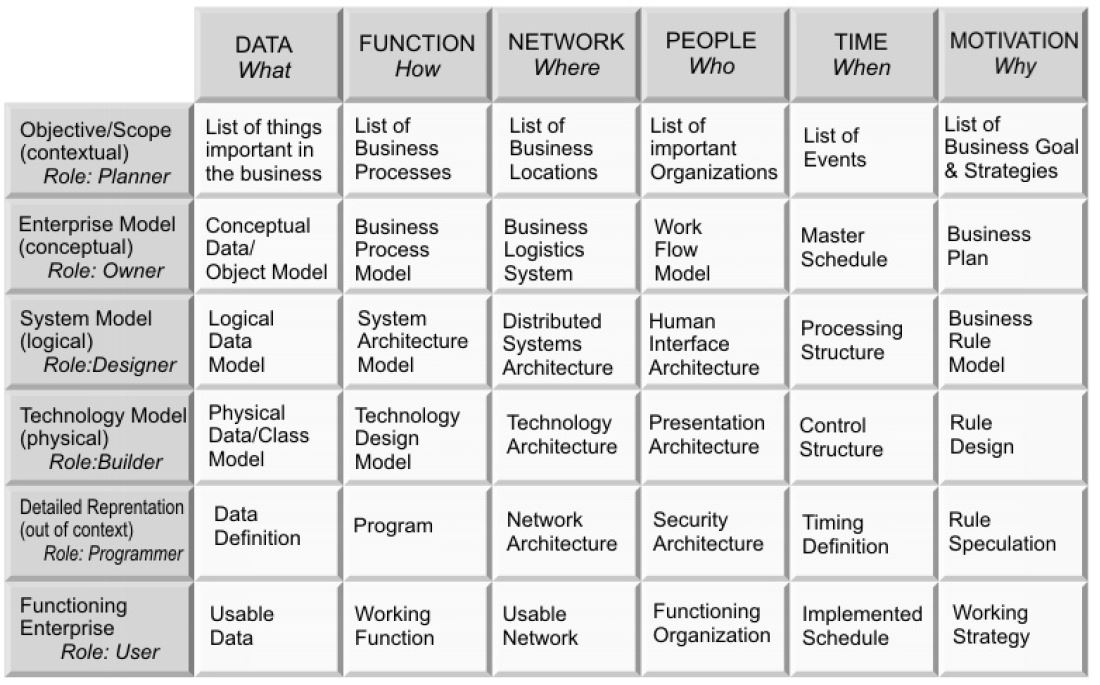
\includegraphics[width=0.7\linewidth]{fig/zachmann-model-neue-darstellung}
\caption{Zachmann Framework - neue Darstellung}
\label{fig:zachmann-model-neue-darstellung}
\end{figure}

\subsection{TOGAF}

\textit{The purpose of enterprise architecture is to optimize across the enterprise the often fragmented legacy of processes (both manual and automated) into an integrated environment that is responsive to change and supportive of the delivery of the business strategy.}

Bekanntestes Architektur-Framework - auch in der Applikations-Architektur.

\begin{figure}[h!]
\centering
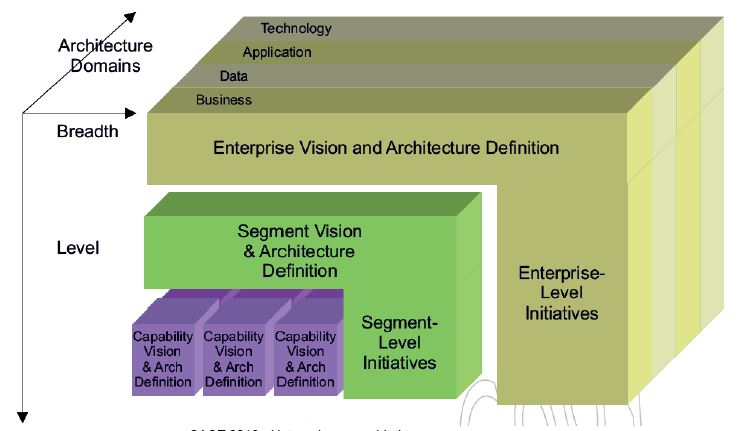
\includegraphics[width=0.7\linewidth]{fig/togaf}
\caption{TOGAF}
\label{fig:togaf}
\end{figure}


\section{Referenzarchitekturen}

\begin{itemize}
	\item Geben einen Rahmen für die Beschreibung von Unternehmensarchitekturen vor
	\item Stellen Methoden zur Verfügung, um Unternehmensarchitekturen zu gestalten und weiterzuentwickeln
	\item Wirken standardisierend
	\item Allgemeine RA (Zachmann Framework, TOGAF)
	\item Industriespezifische RA (TM Forum NGOSS/Frameworks, BIAN Banking Industry Architecture Network)
\end{itemize}

Ein \textbf{Standard} ist eine Vereinbarung zwischen Beteiligten. Einheitliche oder vereinheitlichte, weithin anerkannte und meist auch angewandte (oder zumindest angestrebte) Art und Weise, etwas herzustellen oder durchzuführen. Hat sich gegenüber anderen Arten und Weisen durchgesetzt. Vor allem in der Technik, aber auch Menschenrechte, Umweltschutz. Es ist in einem formalisierten oder nicht-formalisierten Regelwerk beschrieben (Normen).

Eine \textbf{Referenzarchitektur} ist eine IT-Architektur, die standardisierend für die IT-Architekturen einer Gruppe von Informationssystemen wirkt. Diese enthält folgende Elemente:
\begin{itemize}
	\item Definition des Einsatzbereiches
	\item Bausteine, Schnittstellen und Laufzeitstrukturen
	\item Technische Vorgaben zu Software/Hardware
	\item Optional: Vorgaben zu Entwicklungsprozessen
	\item Optional: Referenzimplementationen, aber selten fertige Bausteine
\end{itemize}

Die Verwendung von Referenz-Architekturen führt allgemein zu besserer Architektur und schnellerer Entwicklung (Orientierung und Wiederverwendung). 

Anforderungen an Referenzarchitekturen:
\begin{itemize}
	\item Die Basis sind bewährte Architektur-Mittel
	\item Referenz-Architekturen müssen erfolgreich eingesetzt worden sein, bevor sie diesen Titel tragen
	\item Anpassbarkeit (Ausschnitte müssen verwendbar sein)
	\item Umfassende Dokumentation!
\end{itemize}

Arten von Referenz-Architekturen:
\begin{itemize}
	\item \textbf{Funktionale RA} Fokus auf funktionelle Komponenten und ihre Schnittstellen, ausgehend von Geschäftsprozessen und Services (Frameworks/NGOSS)
	\item \textbf{Logische RA} Definition von Schichten und Komponenten sowie deren Hierarchie- und Kommunikationsbeziehungen (ISO/OSI)
	\item \textbf{Technische RA} Komponenten in Implementierung/Deployment, legen Basistechnologie und Sprache fest (JEE/Java).
\end{itemize}

Wie kommt man zu einer Referenzarchitektur?
\begin{itemize}
	\item Stakeholder Fokus: Im Interesse vieler Beteiligter, Auf dringende Probleme und ihre Klärung konzentrieren, Identifikation von Risiken und Möglichkeiten.
	
	\item Design-Orientiert: Mehr als nur ein Blockdiagramm, Klare Terminologie und konkrete Spezifikationen
	
	\item Systemweite Fragestellungen angehen: Lösungen anbieten, nicht vorschreiben, Optionen offenhalten
\end{itemize}

Erfolgreich standardisieren
\begin{itemize}
	\item Vorhandene Standards wiederverwenden
	\item Wichtige Entscheidungsträger zusammenbringen
	\item Konzentration auf entscheidende Bestandteile der Architektur (Klare Businessvorteile, strategisch wichtig)
	\item Anreize zur Übernahme geben (Vorteile aufzeigen)
\end{itemize}

\subsection{TM Forum Frameworx}

Frameworx/NGOSS ist ein Beispiel einer funktionalen Referenzarchitektur (New Generation Operations Systems and Software). \textit{Programme to provide ways to help Communication Service Providers to manage their business} - mittels Prinzipien und technischen Spezifikationen.

\begin{figure}[h!]
\centering
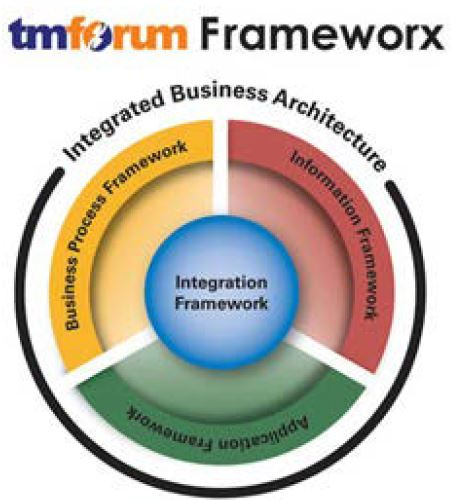
\includegraphics[width=0.7\linewidth]{fig/frameworx}
\caption{Frameworx}
\label{fig:frameworx}
\end{figure}

Das TeleManagement Forum ist ein internationaler Verband der Telekommunikationsbranche. Eine der grössten Industrievereingungen der Welt. Motto: \textit{Enabling the Digital Services Revolution. By providing a neutral and open platform for collaboration between service providers, enterprises and their suppliers, the Forum helps its members overcome the barriers to an open digital economy.}

Das Frameworx/NGOSS enthält eine Referenzarchitektur für die Kernsysteme von Telekommunikations-Anbietern. Basierend auf Service Oriented Architecture (SOA). Behandelt die Gesamt-Architektur inklusive Schnittstellen vom Informationsmodell über die Geschäftsprozesse bis hin zu den angebotenen Diensten. (z. B. Rechnungsstellung oder Freischaltung von SMS für einen Kunden).

\begin{figure}[h!]
\centering
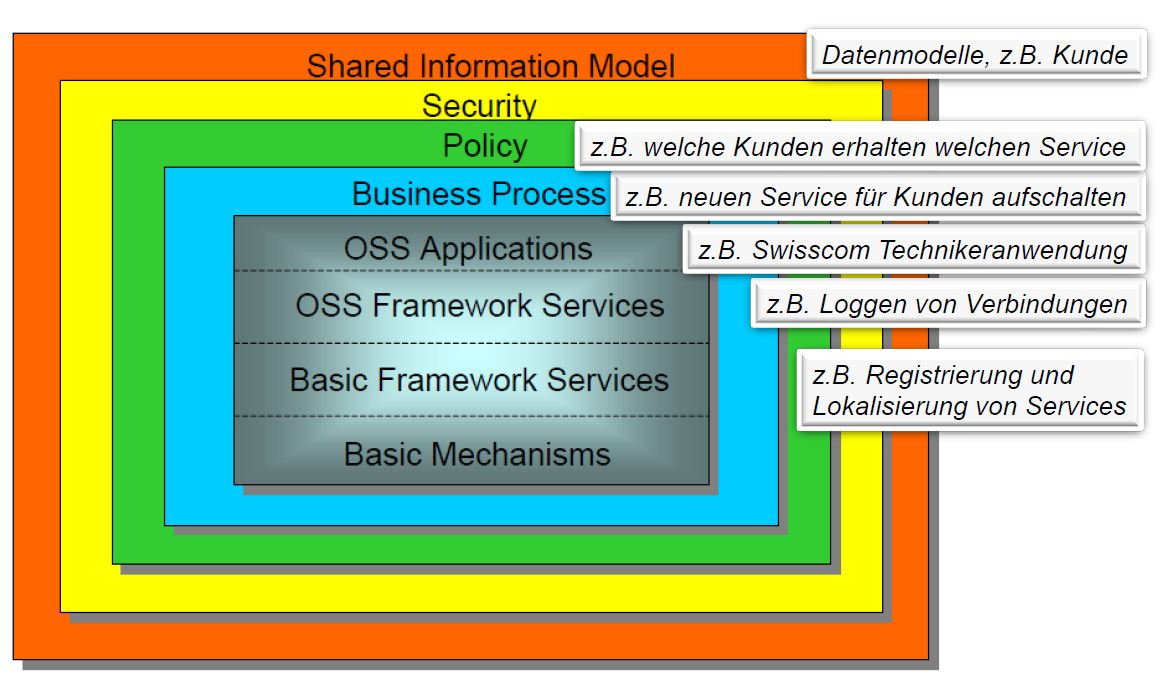
\includegraphics[width=0.7\linewidth]{fig/frameworx-standardisierungsebenen}
\caption{Frameworx Standardisierungsebenen}
\label{fig:frameworx-standardisierungsebenen}
\end{figure}


% Platzhalter EA 3